\documentclass{beamer}

%\documentclass{article}
%\usepackage{beamerarticle}

\usepackage[utf8]{inputenc}

%\usetheme{Warsaw}
%\usetheme{Hannover}
\usetheme{Berkeley}
%\usecolortheme{lily}
\setbeamertemplate{theorems}[numbered] 
%\setbeamertemplate{theorems}[ams style]
\date{}

%\theoremstyle{plain}

\usepackage{lmodern}
\usepackage[T1]{fontenc}
\usepackage[utf8]{inputenc}
\usepackage[french]{babel}
\usepackage{tikz,tkz-tab}
\usepackage{graphics}
\usepackage{pstricks,pst-node,pst-tree}
\usepackage{multicol}
\usepackage{array}


\uselanguage{French}
\languagepath{French}

\newtheorem{proposition}[theorem]{\translate{Proposition}}
\theoremstyle{plain}

%\newtheorem{example}[theorem]{\translate{Example}}
\newtheorem{demonstration}[theorem]{Démonstration}
\newtheorem{remark}[theorem]{Remarque}

\newcommand{\R}{\mathbb{R}}

\title{Produit scalaire}


\begin{document}
  
  \begin{frame}
    
    \titlepage
   % \maketitle
    
  \end{frame}
  
   \section{Angle orienté de vecteurs}
  
  \subsection{Orientation du plan}
 
  \begin{frame}
  

  
  \begin{proposition}
   Tout cercle du plan peut être \uncover<2,3>{orienté} en distinguant sur ce cercle deux sens de parcours. Un sens direct
   et un sens \uncover<3>{indirect}.
 
 \begin{center}
   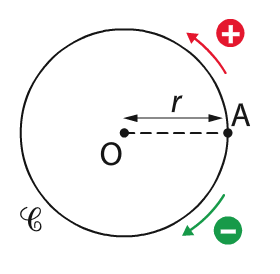
\includegraphics[scale=0.5]{../Images/orientation.png}
 \end{center}
    
  
  \end{proposition}
  
  \end{frame}
  
  \begin{frame}
     On peut orienter tous les cercles du plan de façon cohérente. On dit alors qu'on munit le plan lui-même
    d'une \uncover<2,3,4>{orientation}. Il n'y a que deux orientations du plan possibles. Nous suivrons la convention
    qui consiste à choisir comme sens positif le sens anti-horaire (comme sur le cercle précédent).
    
    On appelle  \textbf{cercle trigonométrique} un cercle \uncover<3,4>{orienté} de rayon \uncover<4>{$1$}. 
  \end{frame}

   \subsection{Angle orienté de vecteurs}

  \begin{frame}
  
  Soient $\vec{u}$ et $\vec{v}$ deux vecteurs non nuls. Soit $\mathcal{C}$ un cercle trigonométrique de 
  centre $O$, $A$ et $B$ les uniques points sur le cercle trigonométrique tels que $\vec{OA}$ 
  (resp. $\vec{OB}$) est colinéaire à $\vec{u}$ (resp. $\vec{v}$).
 
 
  On note $l$ la longueur de l'arc $AB$ parcouru dans le sens direct ($l \geq 0$).

  \begin{center}
    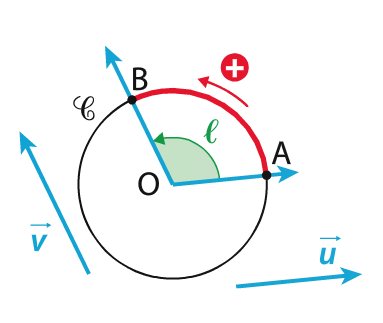
\includegraphics[scale=0.5]{../Images/angleOriente.png}
  \end{center}
  
\end{frame}

\begin{frame}
  \begin{definition}
  Au couple $(\vec{u},\vec{v})$, on associe la famille de nombres réels de la forme 
  $l+\uncover<2,3,4>{2k\pi}, k \in \mathbb{Z}$. Chacun de ces nombres est une mesure de l'\textbf{angle orienté}
   de vecteurs $(\vec{u},\vec{v})$.
   
   L'usage est de noter $(\vec{u},\vec{v})$ un angle de vecteurs et de confondre un angle avec l'une
   de ses mesures. On appelle \textbf{radian} l'\uncover<3,4>{unité de mesure} des angles 
   \uncover<4>{orientés} de vecteurs.

  
  \end{definition}
       \end{frame}
       

\subsection{Mesure principale d'un angle orienté}
 
 \begin{frame}
 \begin{definition}
  \begin{itemize}
   \item Parmi les mesures $x+2k\pi$ de l'angle orienté $(\vec{u},\vec{v})$ de deux vecteurs non nuls,
   il en existe \uncover<2,3,4>{une} et \uncover<3,4>{une seule} dans l'intervalle $]-\pi;\pi]$.
   Cette mesure est appelée la \textbf{mesure 
   principale} de $(\vec{u},\vec{v})$.
   \item On appelle mesure de l'\textbf{angle géométrique} défini par $\vec{u}$ et $\vec{v}$ la valeur
   absolue de la mesure principale de $(\vec{u},\vec{v})$.
  \end{itemize}

 \end{definition}
 \end{frame}

 \begin{frame}
 
  \begin{example} \vspace{0.1cm}~
 
 \begin{itemize}
  \item $\frac{37}{6}\pi=(\uncover<2,3,4,5,6,7,8,9,10,11,12,13>{6}+\frac{1}{6})\pi=\frac{\pi}{6}+
  \uncover<3,4,5,6,7,8,9,10,11,12,13>{3}(2\pi)$. La mesure principale est 
  \uncover<4,5,6,7,8,9,10,11,12,13>{$\frac{\pi}{6}$}.
  \item $\frac{202\pi}{3}=(67+\uncover<5,6,7,8,9,10,11,12,13>{\frac{1}{3}})\pi=\frac{\pi}{3}+67\pi=
  \uncover<6,7,8,9,10,11,12,13>{68\pi} - \pi+\frac{\pi}{3}
  =-\uncover<7,8,9,10,11,12,13>{\frac{2\pi}{3}}
  +\uncover<8,9,10,11,12,13>{34}(2\pi)$. La mesure principale est donc 
  \uncover<9,10,11,12,13>{$-\frac{2\pi}{3}$}.
  L'angle géométrique associé a pour mesure $|-\frac{2\pi}{3}|=\frac{2\pi}{3}$.
  \item Les mesures des angles géométriques en degré et en radian sont proportionnels:
  
  \renewcommand{\arraystretch}{2.2}
 $$
\begin{array}{|c|c|c|c|c|}

\hline
    deg.&180&\uncover<11,12,13>{90}&60&30\\
    \hline
    rad.&\uncover<10,11,12,13>{\pi}&\frac{\pi}{2}&\uncover<12,13>{\frac{\pi}{3}}&\uncover<13>{\frac{\pi}{6}}\\
    \hline
    \end{array} 
$$  
 \end{itemize}

 
 \end{example}
 
 \end{frame}
 
  %\section{Propriétés des angles orientés.}
 
 \subsection{Colinéarité et orthogonalité}
 
 \begin{frame}
 \begin{theorem}
 Soient $\vec{u}$ et $\vec{v}$ deux vecteurs non nuls.
  \begin{itemize}
   \item $(\vec{u},\vec{v})=0$ si et seulement si les vecteurs $\vec{u}$ et $\vec{v}$ sont 
   \uncover<2,3,4,5>{colinéaires}
   et de \uncover<3,4,5>{même sens}.
   \begin{center}
      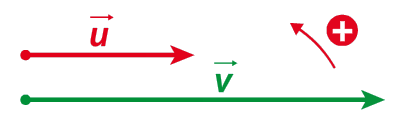
\includegraphics[scale=0.5]{../Images/colMemeSens.png}
   \end{center}

   
   \item $(\vec{u},\vec{v})=\pi$ si et seulement si les vecteurs $\vec{u}$ et $\vec{v}$ sont
   \uncover<4,5>{colinéaires} et de \uncover<5>{sens contraires}.
   \begin{center}
      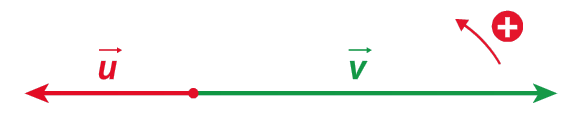
\includegraphics[scale=0.5]{../Images/colSensContraire.png}
   \end{center}
   
  \end{itemize}

 \end{theorem}
 \end{frame}
  
 \begin{frame}
 \begin{definition}
 ~\vspace{-0.5cm}
 
   Les vecteurs $\vec{u}$ et $\vec{v}$ sont \textbf{orthogonaux} si
   $(\vec{u},\vec{v})=\uncover<3,4>{\frac{\pi}{2}}$ ou 
   $(\vec{u},\vec{v})=\uncover<4>{-\frac{\pi}{2}}$.
   \begin{center}
      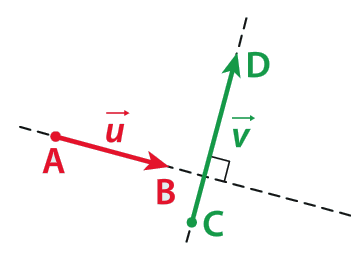
\includegraphics[scale=0.5]{../Images/Ortho.png}
   \end{center}

 \end{definition}
 
 \end{frame}
 
  \subsection{Relation de Chasles}
 
 \begin{frame}
 \begin{theorem}
  Pour tous vecteurs non nuls $\vec{u}$, $\vec{v}$ et $\vec{w}$, on a 
  $(\vec{u},\vec{v})+(\vec{v},\vec{w})=\uncover<2>{(\vec{u},\vec{w})}$.
 \end{theorem}
 \end{frame}
 
 \begin{frame}

 \begin{example}
 \begin{multicols}{2} 
 
  Avec la figure ci-contre:   
  
   $(\vec{BA},\vec{CD})$
   $=(\vec{BA},\uncover<2,3,4,5>{\vec{BC}})+(\uncover<3,4,5>{\vec{BC}},\vec{CD})$
   
   d'où $(\vec{BA},\vec{CD})=\uncover<4,5>{-\frac{3\pi}{4}}+\uncover<5>{\frac{\pi}{3}}=\frac{5\pi}{12}$.
   
   \columnbreak 
   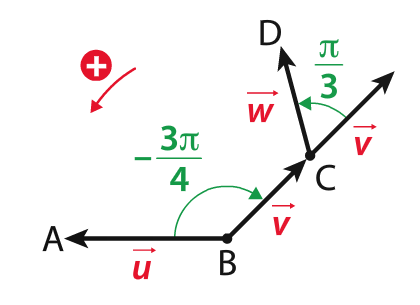
\includegraphics[scale=0.5]{../Images/relChasles.png}
  \end{multicols}

 \end{example}
 \end{frame}
 
 \begin{frame}
  
  \begin{proposition}
 Pour tous vecteurs non nuls $\vec{u}$ et $\vec{v}$:
 \begin{multicols}{2}
  
  
  \begin{center}
    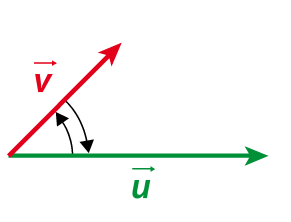
\includegraphics[scale=0.5]{../Images/moinsuv.png}
    
    $(\vec{v},\vec{u})=\uncover<2,3>{-(\vec{u},\vec{v})}$
  \end{center}
 
  
  \columnbreak 
  
  
  \begin{center}
    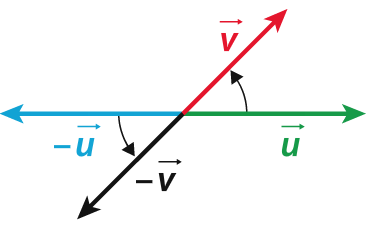
\includegraphics[scale=0.5]{../Images/moinsUetmoinsV.png}
    
    $(-\vec{u},-\vec{v})=\uncover<3>{(\vec{u},\vec{v})}$
  \end{center}

  
  \end{multicols}
  

  
\end{proposition}

\end{frame}

\begin{frame}

\begin{proposition}
 Pour tous vecteurs non nuls $\vec{u}$ et $\vec{v}$:
 \begin{multicols}{2}
  
  \begin{center}
    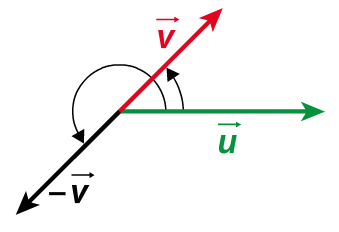
\includegraphics[scale=0.5]{../Images/uMoinsv.png}
    
    $(\vec{u},-\vec{v})=\uncover<2,3>{(\vec{u},\vec{v})+\pi}$
  \end{center}

  
  \columnbreak 

    \begin{center}
    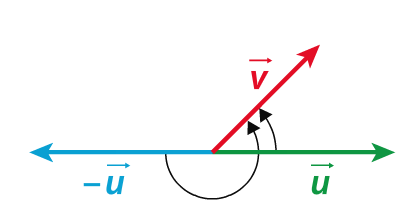
\includegraphics[scale=0.5]{../Images/moinsUetV.png}
    
    $(-\vec{u},\vec{v})=\uncover<3>{(\vec{u},\vec{v})+\pi}$
  \end{center}
  
  \end{multicols}
\end{proposition}

\end{frame}

\begin{frame}

\begin{proposition}
Pour tous vecteurs non nuls $\vec{u}$ et $\vec{v}$
et $k,l>0$, 
 \begin{center}
    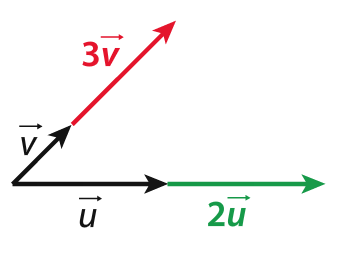
\includegraphics[scale=0.5]{../Images/2u3v.png}
    
    $(k\vec{u},l\vec{v})=\uncover<2>{(\vec{u},\vec{v})}$
  \end{center}
\end{proposition}


 \end{frame}
 
  \section{Produit scalaire}
 
 %\subsection{Norme d'un vecteur}
 
 \begin{frame}
 \begin{definition}
  Une unité de longueur étant choisie, on appelle \textbf{norme} d'un vecteur $\vec{u}=\vec{AB}$
  la longueur $AB$. On note $\|\vec{u}\|=\uncover<2>{\|\vec{AB}\|}=AB$.
 \end{definition}
\end{frame}

 \subsection{Repères orthonormés directs}

 \begin{frame}
 \begin{definition}
  Une unité de longueur étant choisie, dans le plan orienté, on dit que le repère $(O;\vec{i},\vec{j})$
  est \textbf{orthonormé direct} si $\| \vec{i} \|=\| \vec{j}\|=1$ et 
  $(\vec{i},\vec{j})=\uncover<2,3>{\frac{\pi}{2}}$.
  
  Dans un repère orthonormé, si $\vec{u}$ a pour coordonnées $(x;y)$ alors $\|\vec{u}\|=
  \uncover<3>{\sqrt{x^2+y^2}}$.
  
   \begin{center}
    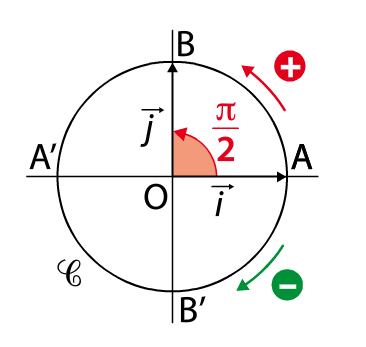
\includegraphics[scale=0.5]{../Images/repereOrthoDirect.png}
  \end{center}
  
 \end{definition}
 
 \end{frame}
 
 \subsection{Trigonométrie}
 \begin{frame}
 
 
 \begin{definition}
 Soient $a$ un angle orienté de vecteurs et $(O;\vec{OA},\vec{OB})$ un repère orthonormé direct. 
 Le \textbf{cosinus} et le \textbf{sinus} de $a$ sont les coordonnées du point $M$ sur un cercle 
 \uncover<2,3,4,5>{trigonométrique} de centre $O$
 tel que $(\uncover<3,4,5>{\vec{OA}},\uncover<4,5>{\vec{OM}})=a$.
  \begin{multicols}{2}
  
  
  \begin{center}
    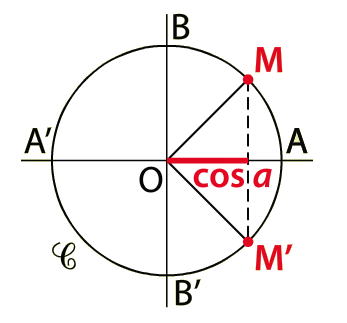
\includegraphics[scale=0.5]{../Images/cosinus.png}
  \end{center}
  
  \columnbreak 
  
  
  \begin{center}
    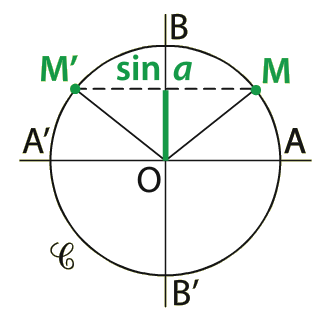
\includegraphics[scale=0.5]{../Images/sinus.png}
  \end{center}

  \end{multicols}
    \begin{center}
   $cos^2(a)+sin^2(a)=\uncover<5>{1}$
  \end{center}
  
 \end{definition}
 \end{frame}
 
 \subsection{Définitions du produit scalaire}
 
 \begin{frame}
 \begin{definition}
  Le \textbf{produit scalaire} de deux vecteurs $\vec{u}$ et $\vec{v}$ est un 
  \uncover<2,3>{nombre réél}. On le note
  $\vec{u}.\vec{v}$ et on lit $\vec{u}$ <<scalaire>> $\vec{v}$. Les définitions suivantes sont équivalentes:
  
  \begin{enumerate}
   \item $\vec{u}.\vec{v}=\frac{1}{2}(\|u+v\|^2-\|\vec{u}\|^2-\|\vec{v}\|^2)$.
   \item $\vec{u}.\vec{v}=\|\vec{u}\|\times\|\vec{v}\|\times cos(\vec{u},\vec{v})$ si $\vec{u}$ et $\vec{v}$ sont non nuls.
   \item $\vec{u}.\vec{v}=xx'+yy'$ si $\vec{u}(x;y)$ et $\vec{v}(x';y')$ dans un repère 
   \uncover<3>{orthonormé}.
  \end{enumerate}
  
 \end{definition}
 \end{frame}

 \subsection{Règles de calcul}
   
 \begin{frame}
 
 
 \begin{proposition}
  Le produit scalaire possède les mêmes propriétés de calcul que le produit de nombres rééls:
  \begin{enumerate}
   \item 
   $\vec{u}.\vec{v}=\uncover<2,3,4,5,6,7>{\vec{v}.\vec{u}}$
    \uncover<3,4,5,6,7>{Commutativité}
   \item $\vec{u}.(\vec{v}+\vec{w})=
   \uncover<4,5,6,7>{\vec{u}.\vec{v}+\vec{u}.\vec{w}}$
    \uncover<5,6,7>{Distributivité}
   \item $(a\vec{u}).(b\vec{v})=\uncover<6,7>{(ab)\vec{u}.\vec{v}}$
    \uncover<7>{Associativité}
  \end{enumerate}

 \end{proposition}
 
 \end{frame}
 
 \begin{frame}
 
  \begin{example}

  \vspace{0.5cm}~
  
  \begin{tabular}{ll}
  %\begin{minipage}[b]{0.47\textwidth}

 $(-\vec{u}).\vec{v}=-\vec{u}.\vec{v}$
 &
 \scriptsize $\vec{AB}.\vec{CD}=-\vec{BA}.\vec{CD}=-\vec{AB}.\vec{DC}$\\
 
 $(\vec{u}+\vec{v})^2=\vec{u}^2+\vec{v}^2+2\vec{u}.\vec{v}$
 &
 \scriptsize $(\vec{AB}+\vec{CD})^2=AB^2+CD^2+2\vec{AB}.\vec{CD}$ \\
  
 $(\vec{u}-\vec{v})^2=\vec{u}^2+\vec{v}^2-2\vec{u}.\vec{v}$
 &
 \scriptsize $(\vec{AB}-\vec{CD})^2=AB^2+CD^2-2\vec{AB}.\vec{CD}$\\
 
 $(\vec{u}+\vec{v})(\vec{u}-\vec{v})=\vec{u}^2-\vec{v}^2$
&
 \scriptsize $(\vec{AB}+\vec{CD})(\vec{AB}-\vec{CD})=AB^2-CD^2$
 
  \end{tabular}

  \end{example}
  
  \end{frame}
 
 %\subsection{Produit scalaire et orthogonalité} 

 \begin{frame}
\begin{theorem}

 Deux vecteurs $\vec{u}$ et $\vec{v}$ non nuls sont orthogonaux si et seulement si \uncover<2,3>{$\vec{u}.\vec{v}=0$}. 
 De même, deux droites $(AB)$ et $(CD)$ sont perpendiculaires si et seulement si 
 \uncover<3>{$\vec{AB}.\vec{CD}=0$}.
\end{theorem}
\end{frame}

\begin{frame}
\begin{proposition}
 Soient $\vec{AB}$ et $\vec{CD}$ deux vecteurs non nuls et $C'$, (resp. $D'$)
 le projeté orthogonal de $C$ (resp. $D$) sur la droite $(AB)$. On a 
 $$\vec{AB}.\vec{CD}=\vec{AB}.\uncover<2>{\vec{C'D'}}$$
 
   \begin{center}
    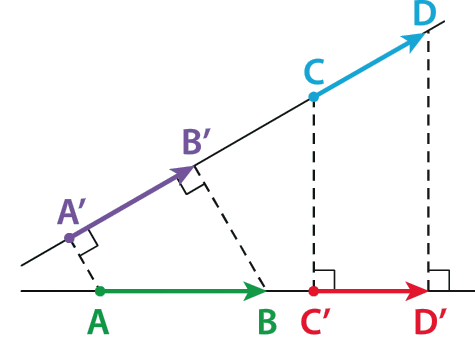
\includegraphics[scale=0.5]{../Images/projetes.png}
  \end{center}
 
 
\end{proposition}
 \end{frame}


 %\section{\'Equations de droites.}
 
 \subsection{Vecteur normal à une droite}

 \begin{frame}
 \begin{definition}
  Un vecteur non nul $\vec{n}$ est \textbf{normal} à une droite $d$ si il est \uncover<2>{orthogonal}
  à tout vecteur directeur de $d$.
  
 \end{definition}
 \end{frame}
 
 \begin{frame}
  \begin{proposition}
  Un point $M$ appartient à la droite $d$ passant par $A$ et perpendiculaire à la droite $(PQ)$
  si et seulement si \uncover<2,3,4>{$\vec{AM}.\vec{PQ}=0}$
  
     \begin{center}
    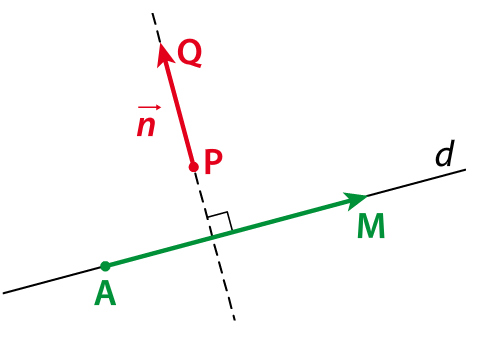
\includegraphics[scale=0.25]{../Images/vecNormal.png}
  \end{center}
  
  Si $d$ et $d'$ sont deux droites de vecteurs directeurs respectifs $\vec{u}$ et $\vec{u'}$ et 
  de vecteurs normaux respectifs $\vec{n}$ et $\vec{n'}$ alors
  $$ d \perp d' \Leftrightarrow \uncover<3,4>{\vec{u}.\vec{u'}=0} \Leftrightarrow 
  \uncover<4>{\vec{n}.\vec{n'}}=0$$
 \end{proposition}
 \end{frame}
 
 \begin{frame}
 \begin{theorem}
  Dans un repère orthonormé:
  \begin{enumerate}
   \item Si une droite $d$ possède une équation de la forme $ax+by+c=0$ avec $a \neq0$ ou
   $b \neq 0$ alors $\vec{n}(a,b)$ est un vecteur \uncover<2,3>{normal} de $d$.
   \item Si un vecteur $\vec{n}(a;b) \neq \vec{0}$ est normal à une droite $d$ alors
   $d$ possède une équation de la forme \uncover<3>{$ax+by+c=0$}.
  \end{enumerate}

 \end{theorem}
 \end{frame}
 
 \begin{frame}
 \begin{example}
  Soient $A(1;2)$, $B(2;5)$ et $C(4;2)$ dans un repère orthonormé. Trouver une équation 
  cartésienne pour la droite $d$ perpendiculaire à $(AB)$ passant par $C$.
  
  $\vec{AB}\uncover<2,3,4,5,6>{(1;3)}$ est un vecteur \uncover<3,4,5,6>{normal} à $d$. 
  $d$ possède une équation de la forme $d:\uncover<4,5,6>{x+3y+c=0}$.
  $C\uncover<5,6>{(4;2)} \in d \Leftrightarrow \uncover<6>{4+3 \times 2+c=0} \Leftrightarrow c=-10$. En définitive,
  $d:x+3y-10=0$.
 \end{example}
 \end{frame}
 
 \subsection{\'Equations de cercles}

 \begin{frame}
\begin{theorem}
 Dans un repère orthonormé, le cercle $\mathcal{C}$ de centre $I(x_0;y_0)$ et de rayon $r$ a
 pour équation $$\mathcal{C}:(x-x_0)^2+(y-y_0)^2=r^2$$
 
      \begin{center}
    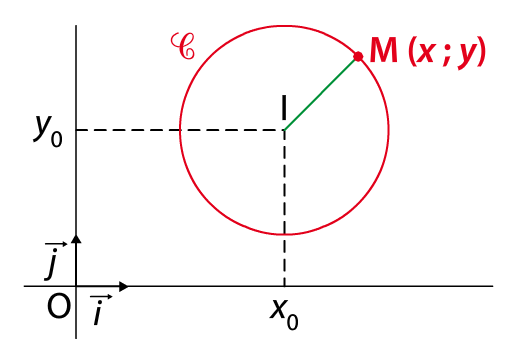
\includegraphics[scale=0.5]{../Images/cercleCentreI.png}
  \end{center}
\end{theorem}

\end{frame}

\begin{frame}
\begin{demonstration}
 $M(x;y) \in \mathcal{C} \Leftrightarrow \uncover<2,3,4,5>{IM^2=r^2} 
 \Leftrightarrow \uncover<3,4,5>{(x-x_0)^2+(y-y_0)^2=r^2}$
\end{demonstration}


\begin{example}
 $(x+1)^2+(y-2)^2=12$ est l'équation d'un cercle de centre $I\uncover<4,5>{(-1;2)}$ et de rayon 
 $r=\uncover<5>{2\sqrt{3}}$.
\end{example}
\end{frame}

\begin{frame}
\begin{theorem}
 $M$ appartient au cercle de diamètre $[AB]$ si et seulement si 
 \uncover<2>{$\vec{AM}.\vec{BM}=0$}.
 
      \begin{center}
    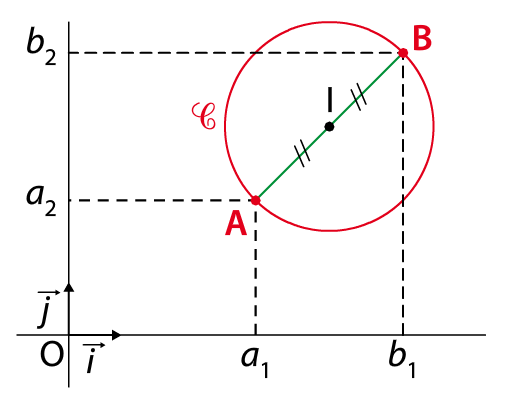
\includegraphics[scale=0.5]{../Images/cercleDiametre.png}
  \end{center}
\end{theorem}
\end{frame}
\begin{frame}
\begin{demonstration}
 Dans un repère orthonormé, $M(x;y)$, $A(a_1;a_2)$ et $B(b_1;b_2)$.
 
 $\vec{MA}.\vec{MB}=0 \Leftrightarrow (x-a_1)(x-b_1)+(y-a_2)(y-b_2)=0$
 
 $\Leftrightarrow [x^2-(a_1+b_1)x]+[y^2-(a_2+b_2)y]=-a_1b_1-a_2b_2$
 
 $\Leftrightarrow [(x-\frac{a_1+b_1}{2})^2-(\frac{a_1+b_1}{2})^2]+[(y-\frac{a_2+b_2}{2})^2-(\frac{a_2+b_2}{2})^2]=-a_1b_1-a_2b_2$
 
 $\Leftrightarrow (x-x_I)^2+(y-y_I)^2=\frac{1}{4}[(a_1+b_1)^2+(a_2+b_2)^2-4a_1b_1-4a_2b_2]=\frac{1}{4}[(b_1-a_1)]^2+(b_2-a_2)^2]=(\frac{AB}{2})^2$
\end{demonstration}
\end{frame}

\subsection{Théorème de Pythagore généralisé}

\begin{frame}
\begin{theorem}
 Soit $ABC$ un triangle quelconque. 
 $$BC^2=\uncover<5>{AB^2+AC^2-2 \times AB\times AC\times cos(\vec{AB};\vec{AC})}$$
 
\end{theorem}

\begin{demonstration}
 $BC^2=\uncover<2,3,4,5>{\vec{BC}^2}=
 \uncover<3,4,5>{(\vec{AC}-\vec{AB})^2}=\uncover<4,5>{AB^2+AC^2-2\times \vec{AB}.\vec{AC}}$
\end{demonstration}
\end{frame}

%\subsection{Théorème de la médiane.}

\begin{frame}
\begin{theorem}
 Soit $ABC$ un triangle quelconque et $I$ le milieu de $[BC]$. $AB^2+AC^2=2AI^2+\frac{BC^2}{2}$
 
   \begin{center}
    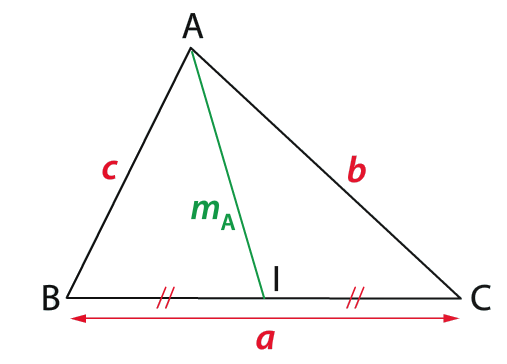
\includegraphics[scale=0.25]{../Images/mediane.png}
  \end{center}
\end{theorem}

\begin{demonstration}
 $AB^2+AC^2=(\uncover<2,3,4,5,6,7,8>{\vec{AI}+\vec{IB}})^2+(\uncover<3,4,5,6,7,8>{\vec{AI}+\vec{IC}})^2$
 $= \uncover<4,5,6,7,8>{2AI^2}+\uncover<5,6,7,8>{2IB^2}+
 2(\uncover<6,7,8>{\vec{AI}.\vec{IB}+\vec{AI}.\vec{IC}})=
 2AI^2+\frac{BC^2}{2}$. 
 
 En effet, $\vec{AI}.\vec{IB}+\vec{AI}.\vec{IC}=\vec{AI}.(\uncover<7,8>{\vec{IB}+\vec{IC}})=
 \vec{AI}.\uncover<8>{\vec{0}}=0$.
\end{demonstration}
\end{frame}


\subsection{Formules trigonométriques}

\begin{frame}
\begin{theorem}
~

 Formules d'addition:
 
 $sin(a+b)=sin(a)\uncover<2,3,4,5,6,7,8,9,10,11,12,13>{cos(b)}+cos(a)\uncover<3,4,5,6,7,8,9,10,11,12,13>{sin(b)}$
 
 $cos(a+b)=cos(a)\uncover<4,5,6,7,8,9,10,11,12,13>{cos(b)}-sin(a)\uncover<5,6,7,8,9,10,11,12,13>{sin(b)}$
 
 $sin(a-b)=\uncover<6,7,8,9,10,11,12,13>{sin(a)cos(b)-cos(a)sin(b)}$
  
 $cos(a-b)=\uncover<7,8,9,10,11,12,13>{cos(a)cos(b)+sin(a)sin(b)}$
 \vspace{0.5cm}
 
 Formules de duplication:
 
 $cos(2a)=\uncover<8,9,10,11,12,13>{cos^2(a)-sin^2(a)}
 =\uncover<9,10,11,12,13>{2cos^2(a)-1}
 =\uncover<10,11,12,13>{1-2sin^2(a)}$
 
 $sin(2a)=\uncover<11,12,13>{2sin(a)cos(a)}$
 \vspace{0.5cm}
 
 Formules de linéarisation:
 
 $cos^2(a)=\uncover<12,13>{\frac{1+cos(2a)}{2}}$
 
 $sin^2(a)=\uncover<13>{\frac{1-cos(2a)}{2}}$
\end{theorem}
\end{frame}
  \iffalse

\fi
   
  %\end{frame}
 
  
\end{document}